\section{Scenario 4C Mixed-Fleet xTM + DAA (eVTOL/UAM Proxy)}
\label{sec:scen4c_mixed_fleet}

This section documents an additional Macro-Scale Strategic Layering Analysis (MSLA) experiment
that approximates the integration of higher-performance Urban Air Mobility (UAM)/eVTOL flows
into the same low-altitude architecture used in the baseline drone scenarios. Scenario~4C reuses
the hybrid stack from Scenario~4B---centralised 4D \gls{xtm} reservations with Python4b-style
tactical logic and stochastic wind perturbations---but replaces the homogeneous sUAS fleet with
a mixed set of performance profiles. The traffic mix combines light and heavy rotorcraft with
light and heavy fixed-wing aircraft, representing higher-mass, higher-speed vehicles that act
as a proxy for future eVTOL/UAM corridor operations under the same BR-xTM governance model.

For parity with the other MSLA experiments, Scenario~4C was evaluated over a \textbf{1-hour}
horizon in the SJC geofence at two traffic densities: \textbf{$N=200$} and \textbf{$N=500$}
physical aircraft. Both runs use the same 20\,m horizontal / 10\,m vertical MACproxy cylinder
and the same GA-tuned DAIDALUS configuration adopted in Scenario~4B. The run directories
\texttt{experiments/xtm\_primordial\_rust/results/run\_200d\_1h} and
\texttt{experiments/xtm\_primordial\_rust/results/run\_500d\_1h} contain per-scenario
\texttt{sim\_metrics.json} files and consolidated \texttt{analysis\_summary.json} outputs used
for the plots and discussion below. Figures were generated with
\texttt{documentation/report\_sections/figures/scen4c\_mixed\_fleet/build\_figures.py}.

\subsection{Quantitative comparison: homogeneous vs.\ mixed fleet at $N=200$}

Table~\ref{tab:scen4c_n200} summarises the key quantitative metrics for Scenarios~4B and 4C at
$N=200$, distinguishing the baseline (geometric DAA only) arm from the DAIDALUS-enabled arm.

\begin{table}[htbp]
\caption{Scenarios 4B and 4C at $N=200$ (1\,h, SJC geofence).}
\label{tab:scen4c_n200}
\begin{center}
\begin{tabular}{|l|l|r|r|r|r|}
\hline
\textbf{Scenario} & \textbf{Arm} & \textbf{MACproxy} & \textbf{DAA pairs} & \textbf{Completion} & \textbf{Ineff.\%} \\
\hline
4B (homog.) & baseline (no DAIDALUS) & 71   & 39   & 862/986  & 2.85 \\
4B (homog.) & + DAIDALUS              & 1337 & 3401 & 718/986  & 47.72 \\
4C (mixed)  & baseline (no DAIDALUS) & 51   & 28   & 882/1002 & 3.28 \\
4C (mixed)  & + DAIDALUS              & 573  & 3808 & 756/1002 & 46.41 \\
\hline
\end{tabular}
\end{center}
\end{table}

From a safety perspective, the mixed-fleet architecture exhibits no degradation relative to the
homogeneous 4B case at the same density. In the baseline arm (hybrid \gls{xtm} + geometric DAA,
without NASA DAIDALUS), the number of MACproxy events remains low and actually decreases from
71 unique violating pairs in Scenario~4B to 51 in Scenario~4C, while the number of completed
missions increases from 862/986 to 882/1002. The modest increase in route inefficiency (from
2.85\,\% to 3.28\,\%) is consistent with the longer mean mission distances and vertical
stratification associated with the higher-altitude fixed-wing/eVTOL proxy profiles.

When the DAIDALUS-based tactical arm is enabled, both scenarios exhibit the expected increase
in alert-driven manoeuvring and route extension, with route inefficiency in the 46--48\,\% band.
However, the mixed-fleet configuration reduces MACproxy from 1337 to 573 unique violating pairs
and increases mission completion from 718/986 to 756/1002 relative to Scenario~4B. This behaviour
is consistent with the introduction of altitude bands and differentiated performance envelopes:
faster, higher fixed-wing/eVTOL-like aircraft are naturally separated in the vertical dimension
and spend less time dwelling in the most saturated low-altitude layers, reducing the effective
conflict graph even though the DAIDALUS monitor flags more alert pairs overall.

\subsection{Quantitative comparison at $N=500$}

Table~\ref{tab:scen4c_n500} extends the same comparison to the higher-density case ($N=500$).

\begin{table}[htbp]
\caption{Scenarios 4B and 4C at $N=500$ (1\,h, SJC geofence).}
\label{tab:scen4c_n500}
\begin{center}
\begin{tabular}{|l|l|r|r|r|r|}
\hline
\textbf{Scenario} & \textbf{Arm} & \textbf{MACproxy} & \textbf{DAA pairs} & \textbf{Completion} & \textbf{Ineff.\%} \\
\hline
4B (homog.) & baseline (no DAIDALUS) & 95307 & 3583  & 2030/2433 & 2.77 \\
4B (homog.) & + DAIDALUS              & 18521 & 26620 & 1344/2433 & 99.85 \\
4C (mixed)  & baseline (no DAIDALUS) & 20400 & 878   & 2135/2453 & 3.72 \\
4C (mixed)  & + DAIDALUS              & 8615  & 36684 & 1343/2453 & 100.63 \\
\hline
\end{tabular}
\end{center}
\end{table}

At $N=500$, the mixed-fleet profile remains favourable relative to homogeneous 4B in terms of
MACproxy count for both tactical arms (4C lower than 4B in baseline and DAIDALUS arms). The
completion ratio in the baseline arm is also slightly higher in 4C (2135/2453) than in 4B
(2030/2433). Under DAIDALUS at this density, completion converges to nearly the same level for
4B and 4C (1344/2433 vs.\ 1343/2453), while route inefficiency increases to approximately
100\,\% for both. This indicates that, at very high density, tactical overhead dominates route
quality independently of fleet mix, but the mixed-fleet architecture still preserves a lower
MACproxy burden.

\subsection{Delta summary (4C relative to 4B)}

To make the comparative trend explicit across densities, Table~\ref{tab:scen4c_delta_summary}
reports percentage deltas of Scenario~4C relative to Scenario~4B for each tactical arm.
Negative MACproxy deltas are favourable (fewer violating pairs), while positive completion-ratio
deltas are favourable (higher mission completion fraction).

\begin{table}[htbp]
\caption{Relative deltas of 4C vs.\ 4B (\%, same tactical arm and density).}
\label{tab:scen4c_delta_summary}
\begin{center}
\begin{tabular}{|l|r|r|r|}
\hline
\textbf{Case} & \textbf{$\Delta$ MACproxy} & \textbf{$\Delta$ completion ratio} & \textbf{$\Delta$ inefficiency} \\
\hline
$N=200$, baseline  & -28.17\% & +0.69\% & +15.16\% \\
$N=200$, +DAIDALUS & -57.14\% & +3.61\% & -2.75\% \\
$N=500$, baseline  & -78.60\% & +4.31\% & +34.49\% \\
$N=500$, +DAIDALUS & -53.49\% & -0.89\% & +0.78\% \\
\hline
\end{tabular}
\end{center}
\end{table}

This summary reinforces two practical conclusions. First, 4C consistently reduces MACproxy
relative to 4B in all tested conditions, with stronger reduction at higher density in the baseline
arm. Second, the cost profile is density- and arm-dependent: in baseline runs, 4C improves completion
but increases route inefficiency; in DAIDALUS runs at $N=500$, completion converges between 4B and 4C
and inefficiency remains near saturation for both, indicating that tactical overhead dominates this
regime.

\subsection{Figures}

The following charts visualise the Scenario~4B vs.\ 4C comparison at $N=200$ and the density
trend from $N=200$ to $N=500$ for baseline and DAIDALUS arms.

\begin{figure}[htbp]
    \centering
    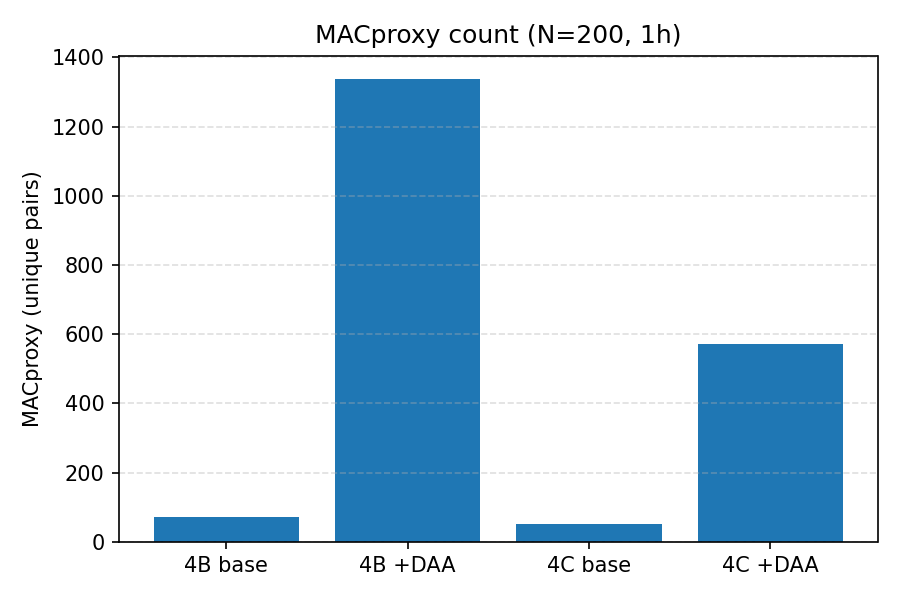
\includegraphics[width=\linewidth]{documentation/report_sections/figures/scen4c_mixed_fleet/fig_scen4c_macproxy_vs_scen.png}
    \caption{MACproxy count for Scenarios 4B and 4C at $N=200$, baseline vs.\ DAIDALUS arms.}
    \label{fig:scen4c_macproxy}
\end{figure}

\begin{figure}[htbp]
    \centering
    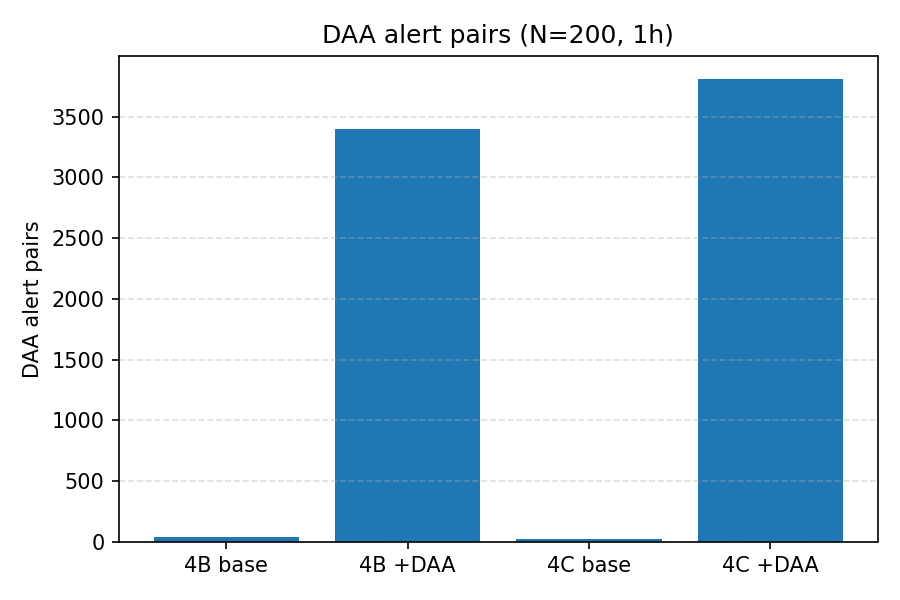
\includegraphics[width=\linewidth]{documentation/report_sections/figures/scen4c_mixed_fleet/fig_scen4c_daa_alert_pairs_vs_scen.png}
    \caption{DAA alert pair count for Scenarios 4B and 4C at $N=200$, baseline vs.\ DAIDALUS arms.}
    \label{fig:scen4c_daa_pairs}
\end{figure}

\begin{figure}[htbp]
    \centering
    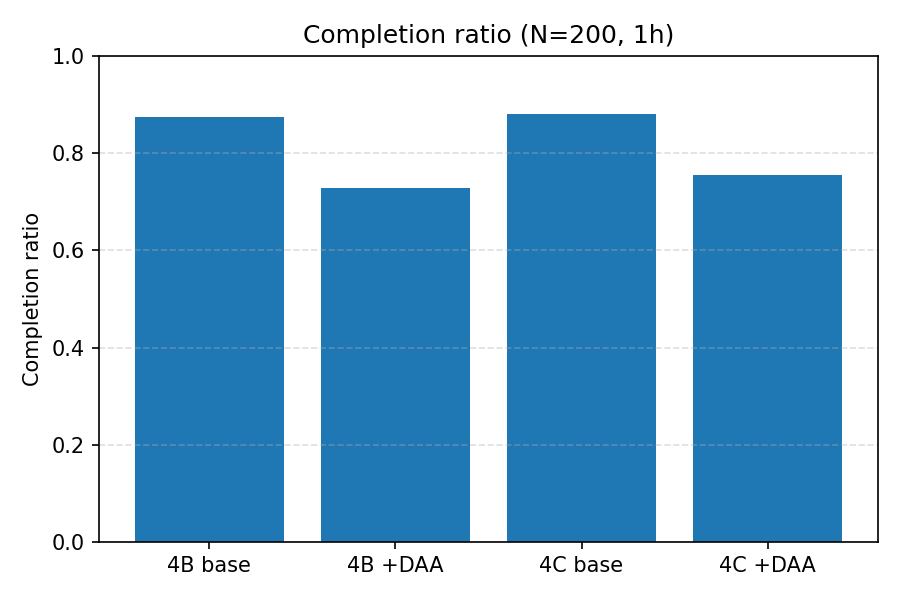
\includegraphics[width=\linewidth]{documentation/report_sections/figures/scen4c_mixed_fleet/fig_scen4c_completion_ratio_vs_scen.png}
    \caption{Completion ratio for Scenarios 4B and 4C at $N=200$, baseline vs.\ DAIDALUS arms.}
    \label{fig:scen4c_completion}
\end{figure}

\begin{figure}[htbp]
    \centering
    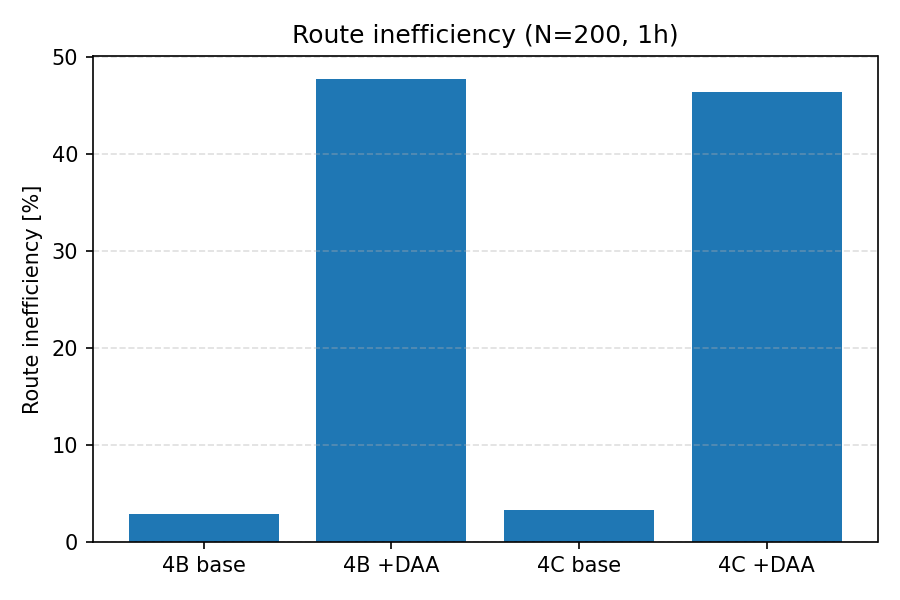
\includegraphics[width=\linewidth]{documentation/report_sections/figures/scen4c_mixed_fleet/fig_scen4c_route_inefficiency_vs_scen.png}
    \caption{Route inefficiency for Scenarios 4B and 4C at $N=200$, baseline vs.\ DAIDALUS arms.}
    \label{fig:scen4c_ineff}
\end{figure}

\begin{figure}[htbp]
    \centering
    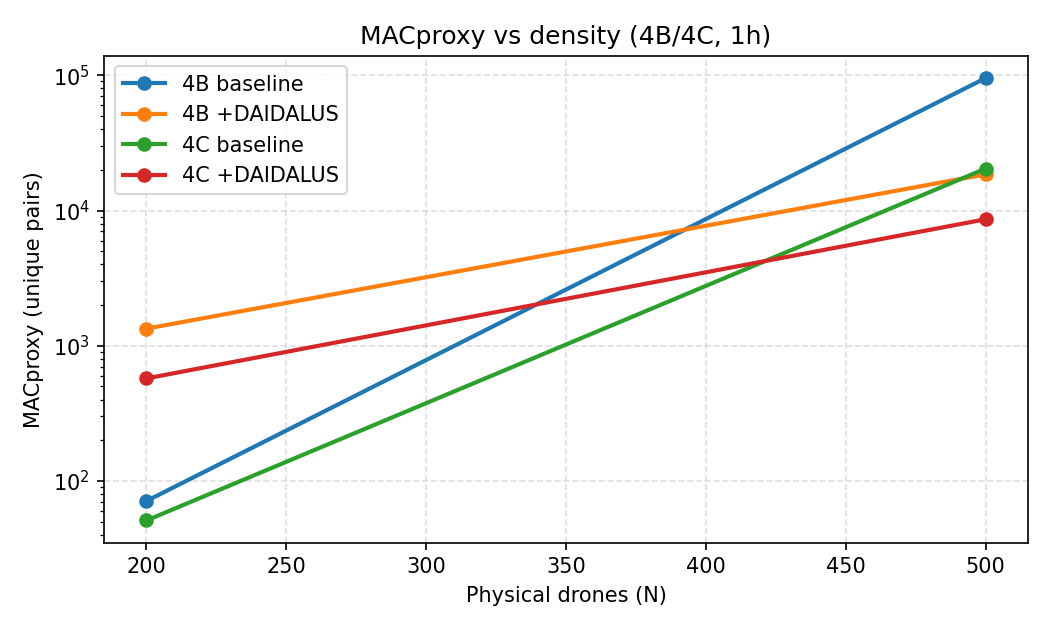
\includegraphics[width=\linewidth]{documentation/report_sections/figures/scen4c_mixed_fleet/fig_scen4c_macproxy_vs_density.png}
    \caption{MACproxy versus density ($N=200$ to $N=500$) for 4B/4C and baseline/DAIDALUS arms (log-scale y-axis).}
    \label{fig:scen4c_macproxy_density}
\end{figure}

\begin{figure}[htbp]
    \centering
    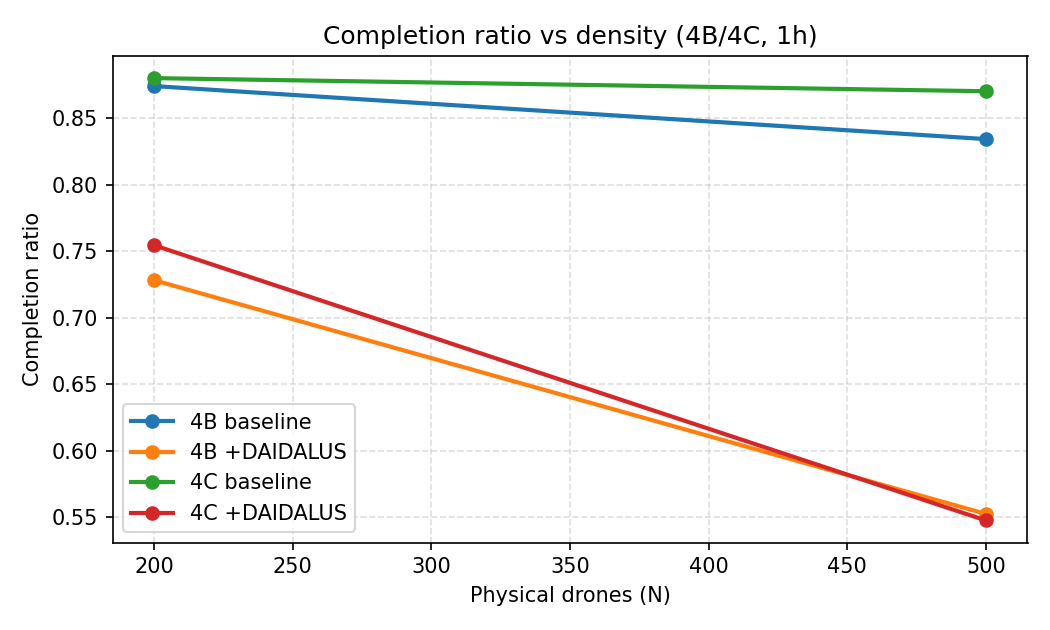
\includegraphics[width=\linewidth]{documentation/report_sections/figures/scen4c_mixed_fleet/fig_scen4c_completion_ratio_vs_density.png}
    \caption{Completion ratio versus density ($N=200$ to $N=500$) for 4B/4C and baseline/DAIDALUS arms.}
    \label{fig:scen4c_completion_density}
\end{figure}

\begin{figure}[htbp]
    \centering
    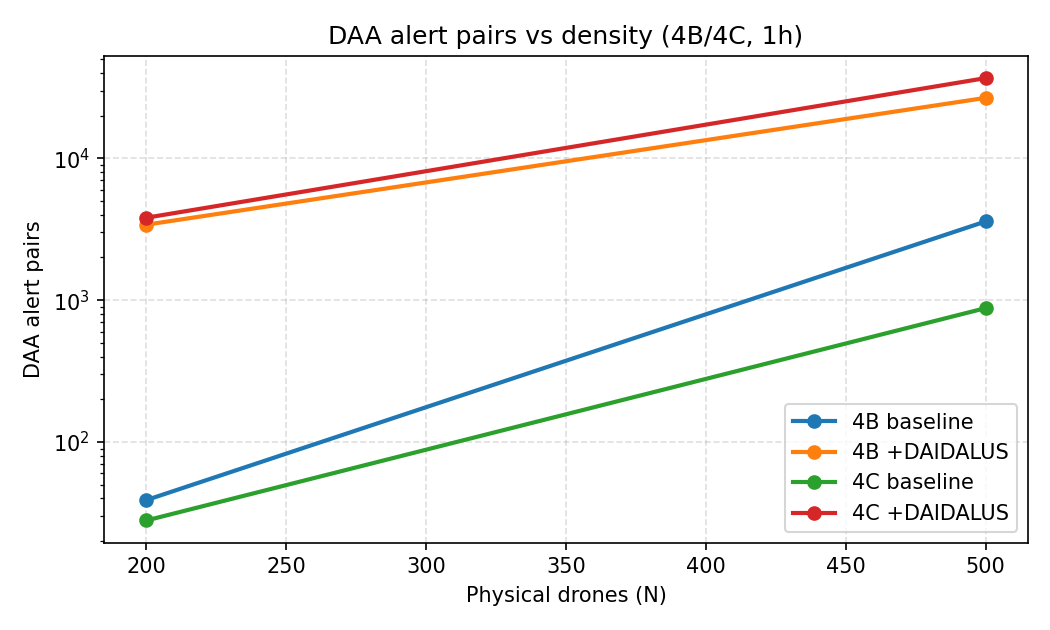
\includegraphics[width=\linewidth]{documentation/report_sections/figures/scen4c_mixed_fleet/fig_scen4c_daa_alert_pairs_vs_density.png}
    \caption{DAA alert-pair counts versus density ($N=200$ to $N=500$) for 4B/4C and baseline/DAIDALUS arms (log-scale y-axis).}
    \label{fig:scen4c_daa_density}
\end{figure}

\begin{figure}[htbp]
    \centering
    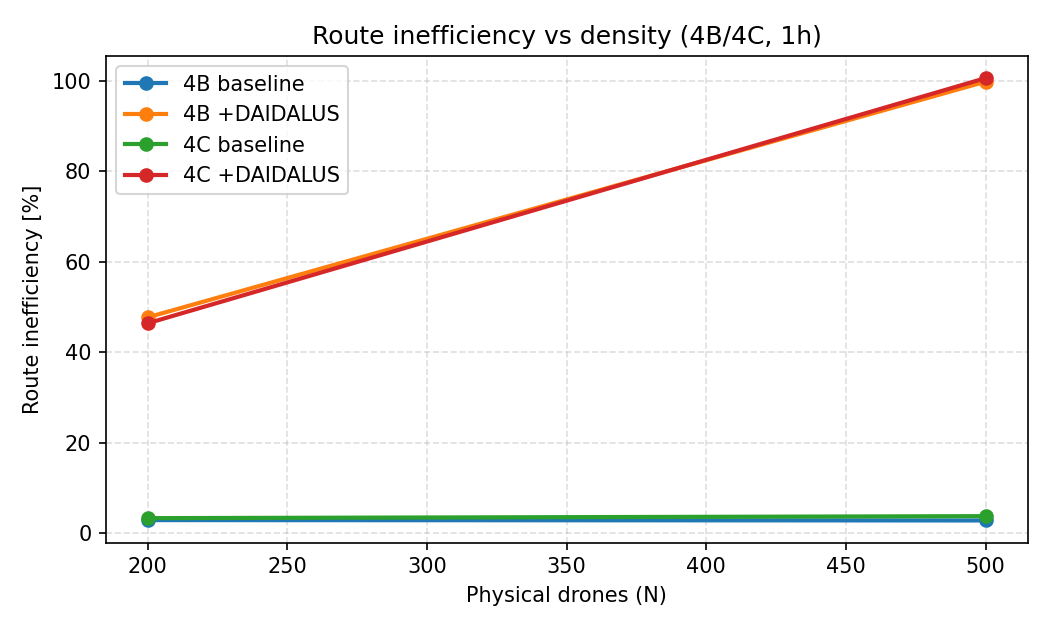
\includegraphics[width=\linewidth]{documentation/report_sections/figures/scen4c_mixed_fleet/fig_scen4c_route_inefficiency_vs_density.png}
    \caption{Route inefficiency versus density ($N=200$ to $N=500$) for 4B/4C and baseline/DAIDALUS arms.}
    \label{fig:scen4c_ineff_density}
\end{figure}

\subsection{Discussion and implications for eVTOL integration}

From an operational-concept standpoint, Scenarios 4C($N=200$) and 4C($N=500$) support the BR-xTM
premise that an architecture validated under conservative sUAS assumptions can generalise to mixed
UAS--eVTOL operations without fundamental changes in the layered logic. The strategic \gls{xtm}
tubes and vertical stratification continue to absorb part of the conflict load, and mixed-fleet
operations remain at least as safe as homogeneous operations under the MACproxy indicator in both
density points.

At the same time, the $N=500$ case shows that conclusions must remain bounded to the tested setup:
single-seed runs and one-hour horizons can expose sharp non-linear transitions (e.g., very large
MACproxy in 4B baseline), and DAIDALUS alert volume does not map one-to-one to MACproxy reduction.
Therefore, the most reasonable conclusion is not that mixed fleets universally ``solve'' density
effects, but that they remain technically compatible with the BR-xTM architecture and can improve
conflict distribution in stressed regimes.

Overall, these experiments provide quantitative evidence that the layered BR-xTM concept, tuned to
ASTM F3442-aligned separation thresholds and equipped with a standardised RWC function, can
accommodate heterogeneous low-altitude fleets without violating the safety rationale established
for purely drone-based operations.

